\chapter{Ist Refactoring immer sinnvoll?}
\section{Beobachten statt vorhersagen}


\chapter{Sicherheit gewinnen, ohne den Code zu verstehen}
Wenn Änderungen an einer Software durchgeführt werden, ist es von hoher Bedeutung, die Sicherheit zu haben, dass danach weiterhin alles funktioniert.
Auch die erfahrensten Entwickler machen hin und wieder Fehler. Fehler sind menschlich.\\
Im folgenden werden einige Maßnahmen vorgestellt, die die Funktionstüchtigkeit von Softwareprojekten gewährleisten können. Insbesondere im Kontext von Refactoring spielt dies eine wichtige Rolle, da dort oft umfassende Änderungen vorgenommen werden. vgl. \citep[S. 323]{fiveLines.2023}
\section{Sicherheit durch Tests}
Die einfachste und verbreitetste Möglichkeit, die Korrektheit von etwas zu überprüfen, ist das Testen. Auch in der Softwareentwicklung ist dies der Fall. Allerdings ist es hier nicht so einfach, wie es sich anhört: Rund die Hälfte der Entwicklungszeit wird in das Testen investiert \citep[Introduction]{artoftesting.2011}.\\
Es gibt viele verschiedene Arten, um Software zu testen, wobei diese sich auf unterschiedlichen Ebenen bewegen. Die folgende Auflistung soll einen Überblick darüber geben. 
\begin{itemize}
  \item \textbf{Unit-Tests} (oder Modultests) sind ein Prozess, bei dem die einzelnen Unterprogramme, Unterroutinen, Klassen oder Prozeduren in einem Programm getestet werden. Genauer gesagt wird der Test nicht zunächst auf das gesamte Programm konzentriert, sondern zuerst auf die kleineren Bausteine des Programms \citep[S. 85]{artoftesting.2011}.
  \item \textbf{Integrations Tests} sollen das Zusammenspiel von einzelnen Modulen, aus dem vorherigen Schritt, testen. Oft ist es der Fall, dass Integrations Tests nicht seperat durchgeführt werden, sondern die Stellen durch umfangreichere Unit-Tests beretis abgedeckt werden \citep[S. 117 f.]{artoftesting.2011}.
  \item \textbf{Funktionale Tests} sind ein Prozess, um Abweichungen zwischen dem Programm und der externen Spezifikation zu finden. Eine externe Spezifikation beschreibt das Verhalten des Programms aus der Sicht des Endbenutzers. Diese Tests werden normalerweise als Black-Box-Test durchgeführt, da das interne Verhalten des Codes in den vorherigen Schritten überprüft wurde. \citep[S. 119]{artoftesting.2011}
\end{itemize}
Diese Liste ist unvollständig, da nur Test-Arten gelistet sind, die den Code direkt betreffen. Es gibt zusätlich noch \textbf{System Tests}, \textbf{Akzeptantz Tests} und \textbf{Installations Tests}. Diese zielen eine höhere Ebene an und sollen die Software als ganzes Testen um festzustellen, ob die angeforderten Problemstellungen des Kunden richtig erfüllt werden und somit z.B.: Missverständnisse bei den Anforderungen ausgeschlossen werden können.
Es ist wichtig zu verstehen, dass diese Ebenen unabhänig voneinander laufen müssen. Funktionieren alle Unit-Tests ordnugnsgemäß, heißt das nicht, dass die Software insgesamt funktioniert, da z.B.: Klassen falsch verwendet werden können.
\textit{„[Außerdem bleibt immer] das Risko, dass unsere Tests genau die Stelle, an der ein Fehler auftritt, nicht abdecken oder dass sie etwas anderes testen, als wir glauben.“} \citep[S. 323]{fiveLines.2023}
\par
Um den Zeitaufwand des Testens auf lange Sicht geringer zu halten, gibt es wie in \citep[S. 323]{fiveLines.2023} die Möglichkeit einige dieser Tests zu automatisieren.
\par
In der modernen Softwareentwicklung sind automatiserte Tests oft Teil einer „Continous Integration“. Dabei muss jeder Commit oder jeder Pull Request vorher definierte Aufgaben erfolgreich absolvieren. Dabei können Unit-Tests, Buildvorgänge \cite{CIMeyer.2014}
\section{Sicherheit durch Werkzeuge}
\begin{wrapfigure}{r}{0.4\textwidth}
  \centering
  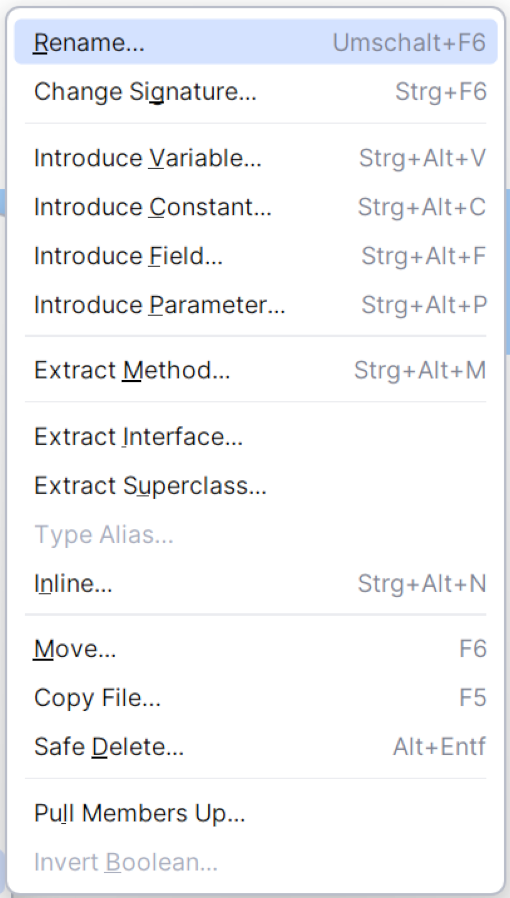
\includegraphics[width=0.35\textwidth]{Bilder/screenshotWebstorm} % Replace with your image file
  \caption{Screenshot WebStorm Refactoring-Tools \cite{webstorm.2024}}
  \label{webstormRefactor}
\end{wrapfigure}
Gerade für Refactorings bieten die meisten modernen Entwicklungsumgebungen verschiedenste Werkzeuge, die den Entwickler unterstützen sollen. In der nebenliegenden Abbildung \ref{webstormRefactor} ist ein Auszug aus den Refactoring-Tools 
\section{Sicherheit durch formale Verifikation}
\section{Sicherheit durch Fehlertoleranz}